\chapter{Why Start Here? Addition and Subtraction}

Addition and subtraction are the building blocks of all mathematical concepts. If we think of math as a language, then addition and subtraction are the alphabet—simple yet powerful tools that help us solve problems, from everyday tasks to complex equations.

Let’s begin by understanding these basic operations deeply. Whether you’re managing your budget, dividing something between friends, or calculating distances, these two operations are always at play.
\begin{center}
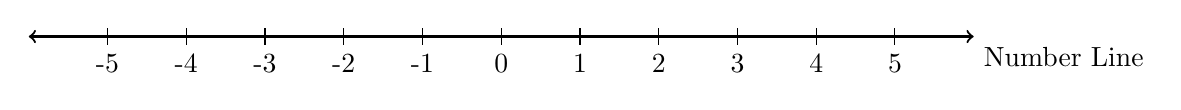
\begin{tikzpicture}
    \draw[thick, <->] (-6,0) -- (6,0) node[anchor=north west] {Number Line};
    \foreach \x in {-5,-4,-3,-2,-1,0,1,2,3,4,5}
        \draw (\x,3pt) -- (\x,-3pt) node[anchor=north] {\x};
\end{tikzpicture}
\end{center}

\section{What Is Addition?}
Addition is the process of combining two or more numbers to get a larger number. Think of it like this:
\begin{itemize}
    \item If you have 3 apples and someone gives you 2 more apples, how many apples do you have in total?
\end{itemize}
This problem is an example of addition: 3 apples + 2 apples = 5 apples.

Let’s look at some other simple examples:
\begin{itemize}
    \item 1 + 1 = 2
    \item 4 + 3 = 7
    \item 10 + 20 = 30
\end{itemize}

Addition works by combining. You start with one number, and as you add more numbers, the total grows.

\subsection{Visualizing Addition}
One of the best ways to understand addition is by using a number line. A number line is a straight line where numbers increase as you move to the right. To add, you simply move to the right by the number you're adding.

For example, if you’re adding 2 + 3, you can start at 2 on the number line and move 3 steps to the right. You’ll land at 5.

\section{What Is Subtraction?}
Subtraction is the process of taking one number away from another. If addition is about combining, subtraction is about removing.

For example:
\begin{itemize}
    \item You have 5 apples, and you give 2 away. How many apples are left?
\end{itemize}
This is subtraction: 5 apples - 2 apples = 3 apples.

Other simple examples:
\begin{itemize}
    \item 7 - 4 = 3
    \item 10 - 5 = 5
    \item 15 - 9 = 6
\end{itemize}

Subtraction helps us find out how much is left or how much we need to remove from something.

\subsection{Visualizing Subtraction}
We can also use a number line for subtraction. Instead of moving to the right as we do with addition, we move to the left.

If you’re subtracting 5 - 2, you start at 5 on the number line and move 2 steps to the left. You’ll land at 3.

\section{Practice Makes Perfect: Let’s Try Some Exercises!}
\subsection{Simple Addition}
\begin{enumerate}
    \item 5 + 4 = \_\_\_\_
    \item 7 + 2 = \_\_\_\_
    \item 10 + 6 = \_\_\_\_
\end{enumerate}

\subsection{Simple Subtraction}
\begin{enumerate}
    \item 8 - 3 = \_\_\_\_
    \item 12 - 5 = \_\_\_\_
    \item 20 - 9 = \_\_\_\_
\end{enumerate}

Try to use a number line for these problems. Draw one out, and for each addition problem, move right. For each subtraction problem, move left. This will help you visualize the process.

\section{Making It Real: Addition and Subtraction in Everyday Life}
Math is everywhere. You use addition and subtraction more often than you think:
\begin{itemize}
    \item \textbf{Shopping:} You bought 3 oranges and added 2 apples to your basket. How many pieces of fruit do you have? That’s 3 + 2 = 5!
    \item \textbf{Cooking:} You have 4 cups of flour, but your recipe only calls for 2 cups. How much flour will you have left after using what you need? That’s 4 - 2 = 2 cups left.
    \item \textbf{Traveling:} You traveled 15 miles, but your destination is 20 miles away. How many miles are left to go? That’s 20 - 15 = 5 miles left.
\end{itemize}

Addition and subtraction help you organize, plan, and make decisions in your daily life.

\section{The Properties of Addition and Subtraction}
Now that we’ve mastered the basics, let’s look at some important properties that will help us understand these operations even better:

\subsection{Commutative Property of Addition}
\begin{itemize}
    \item When adding two numbers, the order doesn’t matter.
    \item For example, 3 + 5 is the same as 5 + 3. Both equal 8.
\end{itemize}

\subsection{Associative Property of Addition}
\begin{itemize}
    \item When adding three or more numbers, it doesn’t matter how you group them.
    \item For example, (2 + 3) + 4 = 2 + (3 + 4). Both equal 9.
\end{itemize}

\subsection{Subtraction is not Commutative}
\begin{itemize}
    \item Unlike addition, the order does matter in subtraction.
    \item For example, 5 - 3 is not the same as 3 - 5. One equals 2, and the other equals -2.
\end{itemize}

\section{Breaking It Down: How to Approach Word Problems}
One of the most important ways math shows up in real life is through word problems. Word problems take a real-world situation and ask you to solve it with math.

Here’s a simple strategy to help you:
\begin{enumerate}
    \item Read the problem carefully.
    \item Identify what you’re being asked to find.
    \item Translate the words into numbers (e.g., “two more” means +2).
    \item Write down the math problem.
    \item Solve it!
\end{enumerate}

Let’s try an example:
\begin{itemize}
    \item \textbf{Problem:} Sarah has 5 marbles. She finds 3 more marbles. How many marbles does Sarah have now?
    \item \textbf{Step 1:} Identify what we know.
    \begin{itemize}
        \item Sarah starts with 5 marbles.
        \item She finds 3 more.
    \end{itemize}
    \item \textbf{Step 2:} Write the math problem:
    \begin{itemize}
        \item 5 + 3 = 8.
    \end{itemize}
    \item \textbf{Step 3:} Solve it. Sarah now has 8 marbles.
\end{itemize}

\section{Chapter Summary}
\begin{itemize}
    \item Addition is about combining numbers to get a larger total.
    \item Subtraction is about removing numbers to see how much is left.
    \item We can use number lines to help visualize both operations.
    \item These operations are useful in everyday life, from shopping to cooking and traveling.
    \item We learned the commutative and associative properties for addition and why subtraction doesn’t have these properties.
\end{itemize}

Mastering addition and subtraction will set the stage for learning more advanced math concepts in the next chapters. Keep practicing, and soon you’ll be ready for the next step: multiplication and division!

\section{Challenge Question}
You have 10 apples. You give 4 apples to your friend, and then you buy 5 more apples. How many apples do you have now?
\begin{equation*}
(10 - 4) + 5 = \_\_\_\_?
\end{equation*}
